\chapter{LDA of Investments in the United States} 
\section{Introduction}
\nocite{tmpackage} \nocite{LDAvis} \nocite{Stargazer}
\nomenclature{MPT}{Modern Portfolio Theory}	

- Now that we know where they are, let's look at how they invest, and why certain regions are specializing in certain sectors.  

While Modern Portfolio Theory (MPT), as established by \cite{Markowitz1952} advocates for holding a broad and negatively correlated portfolio, the notion of "not putting all of one's eggs in a single basket" is an old one, for \cite{Lofthouse53} finds that such advice was practised by the British investment firm Investment Registry as far back as 1904.  

In concert with MPT's emphasis on diversification, the reaction to the Crash of October 1987 placed renewed emphasis on risk management and the rise of ``Value at Risk'' (VAR) based investing in which firms would try to maximise returns while minimizing risk.  This led to a homogenizing effect in investment strategies, as explained by Andrew G. Haldane, executive director of the Financial Stability at the Bank of England at a conference on risk management:

\nomenclature{VAR}{Value at Risk}
\begin{quote}
	Within the financial sector, diversity appears to have been reduced for two separate, but related, reasons:  the pursuit of return;  and the management of risk.  The pursuit of yield resulted in a return on equity race among all types of financial firm.  As they collectively migrated to high-yield activities, business strategies came to be replicated across the financial sector.  Imitation became the sincerest form of flattery.
	
	So savings cooperatives transformed themselves into private commercial banks.  Commercial banks ventured into investment banking.  Investment banks developed in-house hedge funds through large proprietary trading desks.  Funds of hedge funds competed with traditional investment funds.  And investment funds - pension, money market mutual, insurance - imported the risk the others were shedding.   \citep{Haldane2009}[p.18]
\end{quote} 

As explored in Chapter \ref{ChapterII}, there is a substantial literature showing that stock pickers are biased towards industries in which they are knowledgeable, or have personal connections.  According to \cite{covalthe2001}, investors can draw abnormal returns from local knowledge, and another study makes a compelling case that stock pickers are biased towards selecting stocks of companies that their board of directors contain shared alumni networks \citep{Cohen2008} .  

Therefore rather than looking at geographic differences of investors based on the type of institution they belong to, this will attempt to create a functional portfolio archetype, aggregate these archetypes by geography and look for patterns of differences.   
	
\section{Latent Dirichlet allocation}

\nomenclature{LDA}{Latent Dirichlet allocation}
	
Latent Dirichlet allocation (LDA) \nomenclature{LDA}{Latent Dirichlet allocation} is a generative statistical technique developed by David \cite{blei2003latent} to find themes that are common across a corpus of texts.  This technique is a derivation and refinement of \cite{Papadimitriou98} and \cite{PAPADIMITRIOU2000217} work on Latent Semantic Indexing.  

From their origin in text analysis such as analysing 18th century American newspapers for the topics of the day \citep{newman2006probabilistic},  finding topics of controversy and or debate at an academic conference via Twitter usage by the participants of the conference\citep{Marwick2013}, LDA can now be seen in multiple different fiels such as latent patterns in biodiversity data \citep{Vale2014}, and genetic data, images,and social networks \citep{Blei2012}.  Also Satelite images \cite{Lienou2010}

- LDA assumes that language is a "bag of words".  That means that the order of words isn't considered.  For our purpose of using LDA on stock portfolio, the relative ordering of the stocks has zero effect on the output, just the amount of each stock.  

Suppose the following 5 sentences taken from Edwin Chen's introduction to LDA blogpost \cite{Chen2011}.

	\begin{enumerate}
		\singlespacing 
		\item I like to eat broccoli and bananas.
		\item I ate a banana and spinach smoothie for breakfast.
		\item Chinchillas and kittens are cute.
		\item My sister adopted a kitten yesterday.
		\item Look at this cute hamster munching on a piece of broccoli.
	\end{enumerate}

If we were to suppose that we were to limit ourselves to 2 topics, we would see something to the effect of the following:


	\begin{itemize}
	\item \textbf{Sentences 1 and 2:} 100\% Topic A
	\item \textbf{Sentences 3 and 4:} 100\% Topic B
	\item \textbf{Sentence 5:} 60\% Topic A, 40\% Topic B
	\item \textbf{Topic A:} 30\% broccoli, 15\% bananas, 10\% breakfast, 10\% munching, etc... (at which point, you could interpret topic A to be about food)
	\item \textbf{Topic B:} 20\% chinchillas, 20\% kittens, 20\% cute, 15\% hamster, etc...  (at which point, you could interpret topic B to be about cute animals)
	\end{itemize}


A closer analogue to using LDA is using this technique to classifying card selection in games such as Magic:The Gathering \citep{Hlynsson2017}.  This collectible card game uses 60 cards decks that are selected ahead of time.  Due the game's complex resource system and multiple different strategies for attacking one's opponent, cards are not fungible, and thus the game consolidates towards certain discreet collection of cards.  Similarly, the use LDA cab be used to aggregate different stock portfolios into different investment strategies strategies.  

\section{number of topics}
LDA requires the user to determine \textit{a priori} the number of topics used in the Topic Model.  This leads to the lumper vs splitter problem.  Where one has to classify $n$ objects, the optimal number of categories will exist between 1 and $n$, for one category encompasses the ensemble of things to be classified, and $n$ categories will have perfect fit, but is utterly meaningless since it does not reduce data into a meaningful form.  As such, classification is an art as well as a science, since many categories can exist as part of a continuum.

In this case, the optimal number of topics selected was facilitated by the R package LDAtuning \citep{LDAtuning}. This package takes the Document-Term matrix and runs an ensemble of 4 different information criteria in order to find the optimal number of topics.  These are \cite{Arun2010} \cite{CAO2009} \cite{Griffiths2004} and \cite{deveaud2014}.  The suggested number of topics as suggested by \cite{LDAtuning} (Figure \ref{fig:topicselection})is when the differences between of \cite{CAO2009} and \cite{Arun2010} and \cite{Griffiths2004} and \cite{deveaud2014} are minimized.  Looking for numbers of topics where the difference it minimized, one can see such areas at 8, 14, 34 and 72.   However, 8 and 14 offer a poor fit under \cite{Griffiths2004}, and this method suggest a much larger optimal number.  By contrast, \cite{CAO2009} and \cite{deveaud2014} suggest topics at 8, 14 and 34, with \cite{deveaud2014} offering poorer solutions as the number of topics increases.  As such, 34 topics offers the best concillience between the different  tuning methods. 

Model used 34 topics. Due to computing constraints (32gb of ram), the model could only train model on all positions worth more than 1 million dollars USD.  34 Topics was a the limit of computing power and explanatory power.  More topics would have led to more differentiation between topics, but at the cost of creating more niche topics.  As it currently stands, most firms a mix of 3 to four strategies accounting for about 20\% each of their portfolio. 
	
\begin{figure}
	\centering
	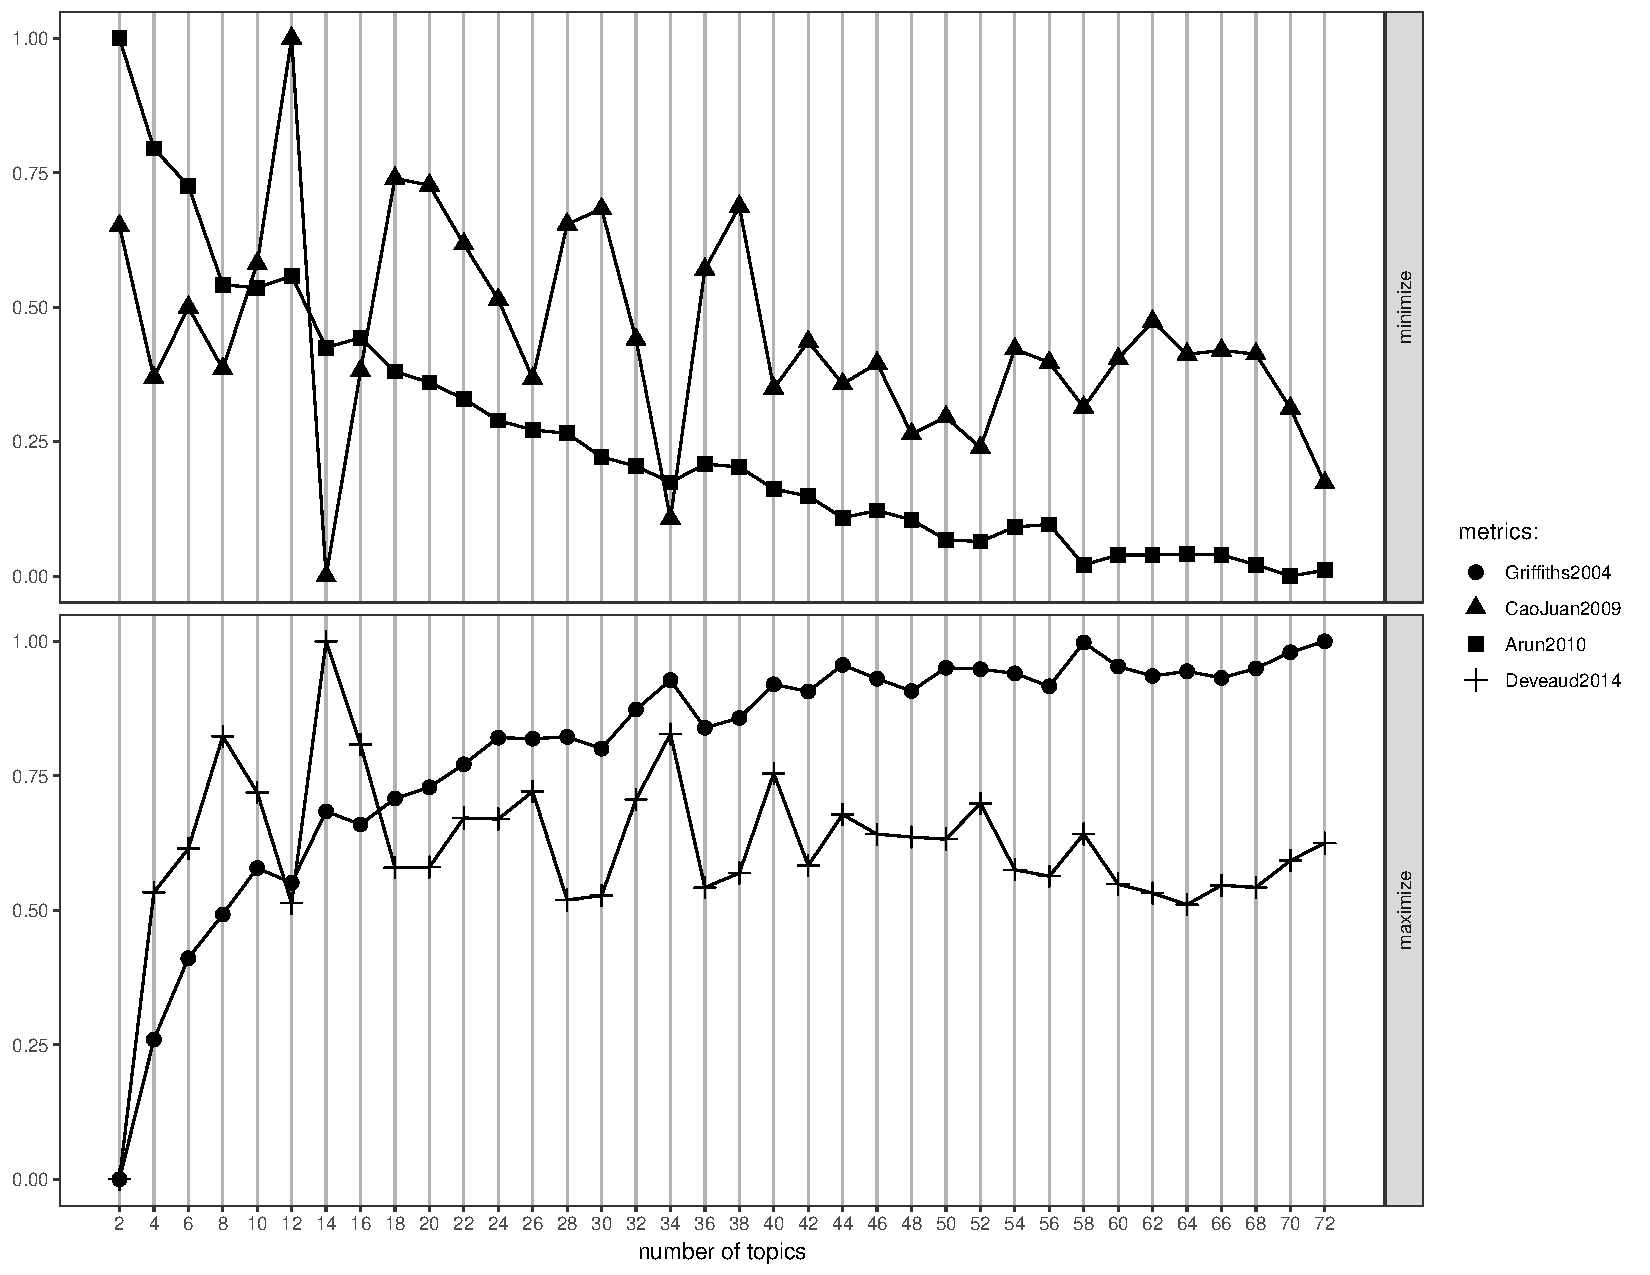
\includegraphics[width=1\linewidth]{Figures/ChapterV/TopicSelection}
	\caption[LDAtuning Ensemble for Determining the Number of Topics in LDA]{LDAtuning Ensemble for Determining the Number of Topics in LDA.   As can be seen from the short distance between Deveaud(2014) and CaoJuan(2009) around 14 topics and the close agreement between the Griffiths(2004) and Arun(2010) measure as the number of topics increases - especially after 58.  This suggests that a number of topics should be between 14 and 58.  within  this band, all 4 metrics are in closest agreement at 34 topics, therefore 34 topcis will be used in the LDA analysis.    }
	\label{fig:topicselection}
\end{figure}
	

	
LDA implementation with \cite{topicmodels}, and text was prepared with the tidytext package \cite{tidytext}.  It should be noted that the order of each topic's number is arbitrary. 
	
\section{Topic Model Results}
	
\begin{figure}
	\centering
	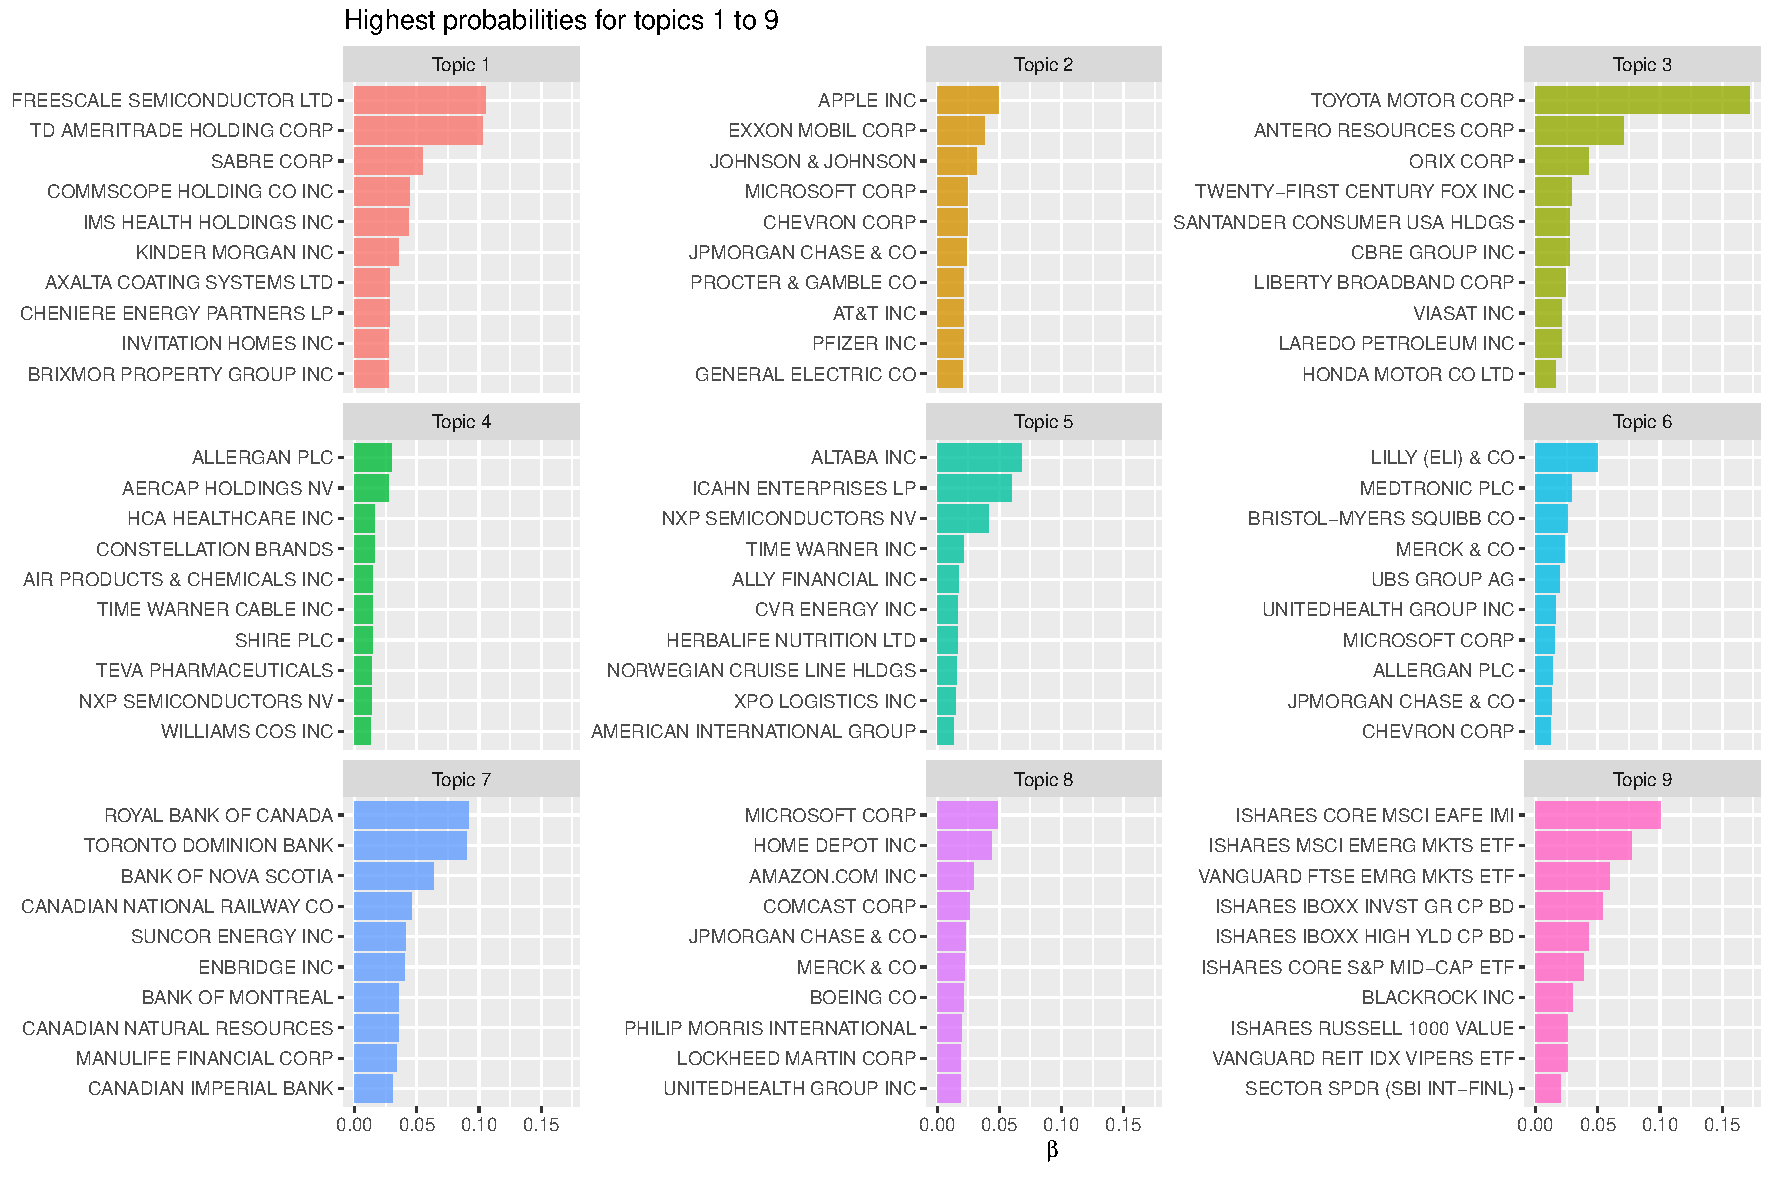
\includegraphics[width=\linewidth]{Figures/ChapterV/LDA34_1-9}
	\caption[Topic Model with 34 Topics, Topics 1 thought 9]{Topic Model with 34 Topics, Topics 1 thought 9. This represents the 10 most likely stocks being associated to a particular portfolio archetype.}
	\label{fig:lda341-9}
\end{figure}

Figure \ref{fig:lda341-9} contains the top 10 stocks to be associated with portfolio archetypes 1 though 9.  Using topic 1 as an example, this topic contains a mix of tech stocks (Microsoft and Intel), pharmaceutical stocks (Pfizer, Merck and Sanofil), banks (JP Morgan,  Wells Fargo and Citigroup) as well as fossil fuel firms such as (Royal Dutch Shell and BP).  That being said, some topics can appear to be quite similar to each other, but a surface level similarity can mask deeper differences.  For example, \nomenclature{ETF}{exchange traded funds} Topics 2, 3, 20 and 29 are quite heavily invested in exchange traded funds (ETF) that index the broader stock market.  The major differences appear to be on the level of ETF diversity as well as the ``hedge'' positions that balance out the rest of the portfolio.  The same can be said for topics 25 and 26 (Figure \ref{fig:lda341927}). These two topics appear quite similar, with a primary difference being primarily about the degree of concentration in Berkshire Hathaway stock, as well as the distribution of the balance of their portfolio.  

Often these parings are a mix and match picking 2 or 3 of the following: Dow Jones Industrial Average-listed stocks, technology stocks, pharmaceutical stocks, financial institutions and energy companies. This is suggestive that depending one's stance on the lumper-spliter debate, one can advocate for as little as 8 topics if one's a lumper, or as many as 72 if one's a splitter and has access to the computing resources to do so.  

\begin{figure}
	\centering
	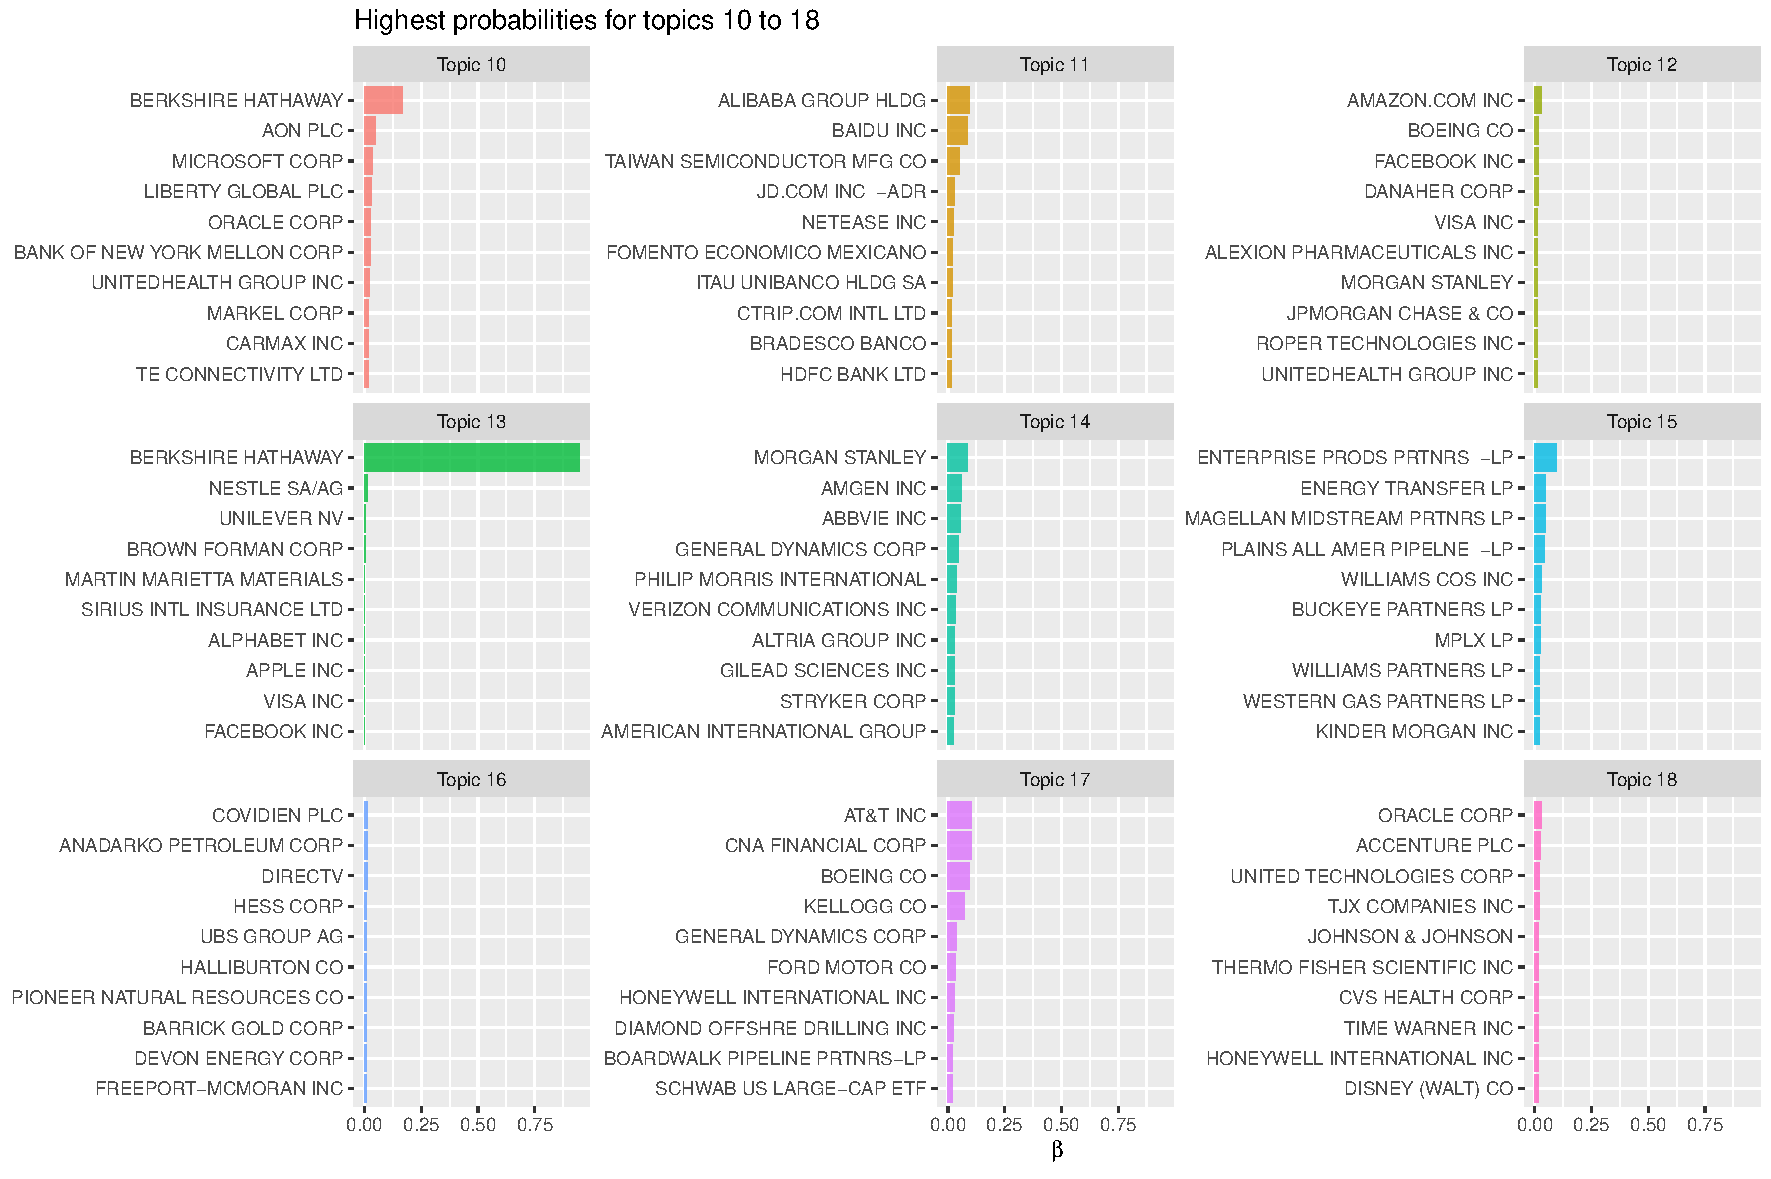
\includegraphics[width=1\linewidth]{Figures/ChapterV/LDA34_10_18}
	\caption[Topic Model with 34 Topics, Topics 10 thought 18]{Topic Model with 34 Topics, Topics 10 thought 18. This represents the 10 most likely stocks being associated to a particular portfolio archetype.}
	\label{fig:lda341018}
\end{figure}
	
	
\begin{figure}
	\centering
	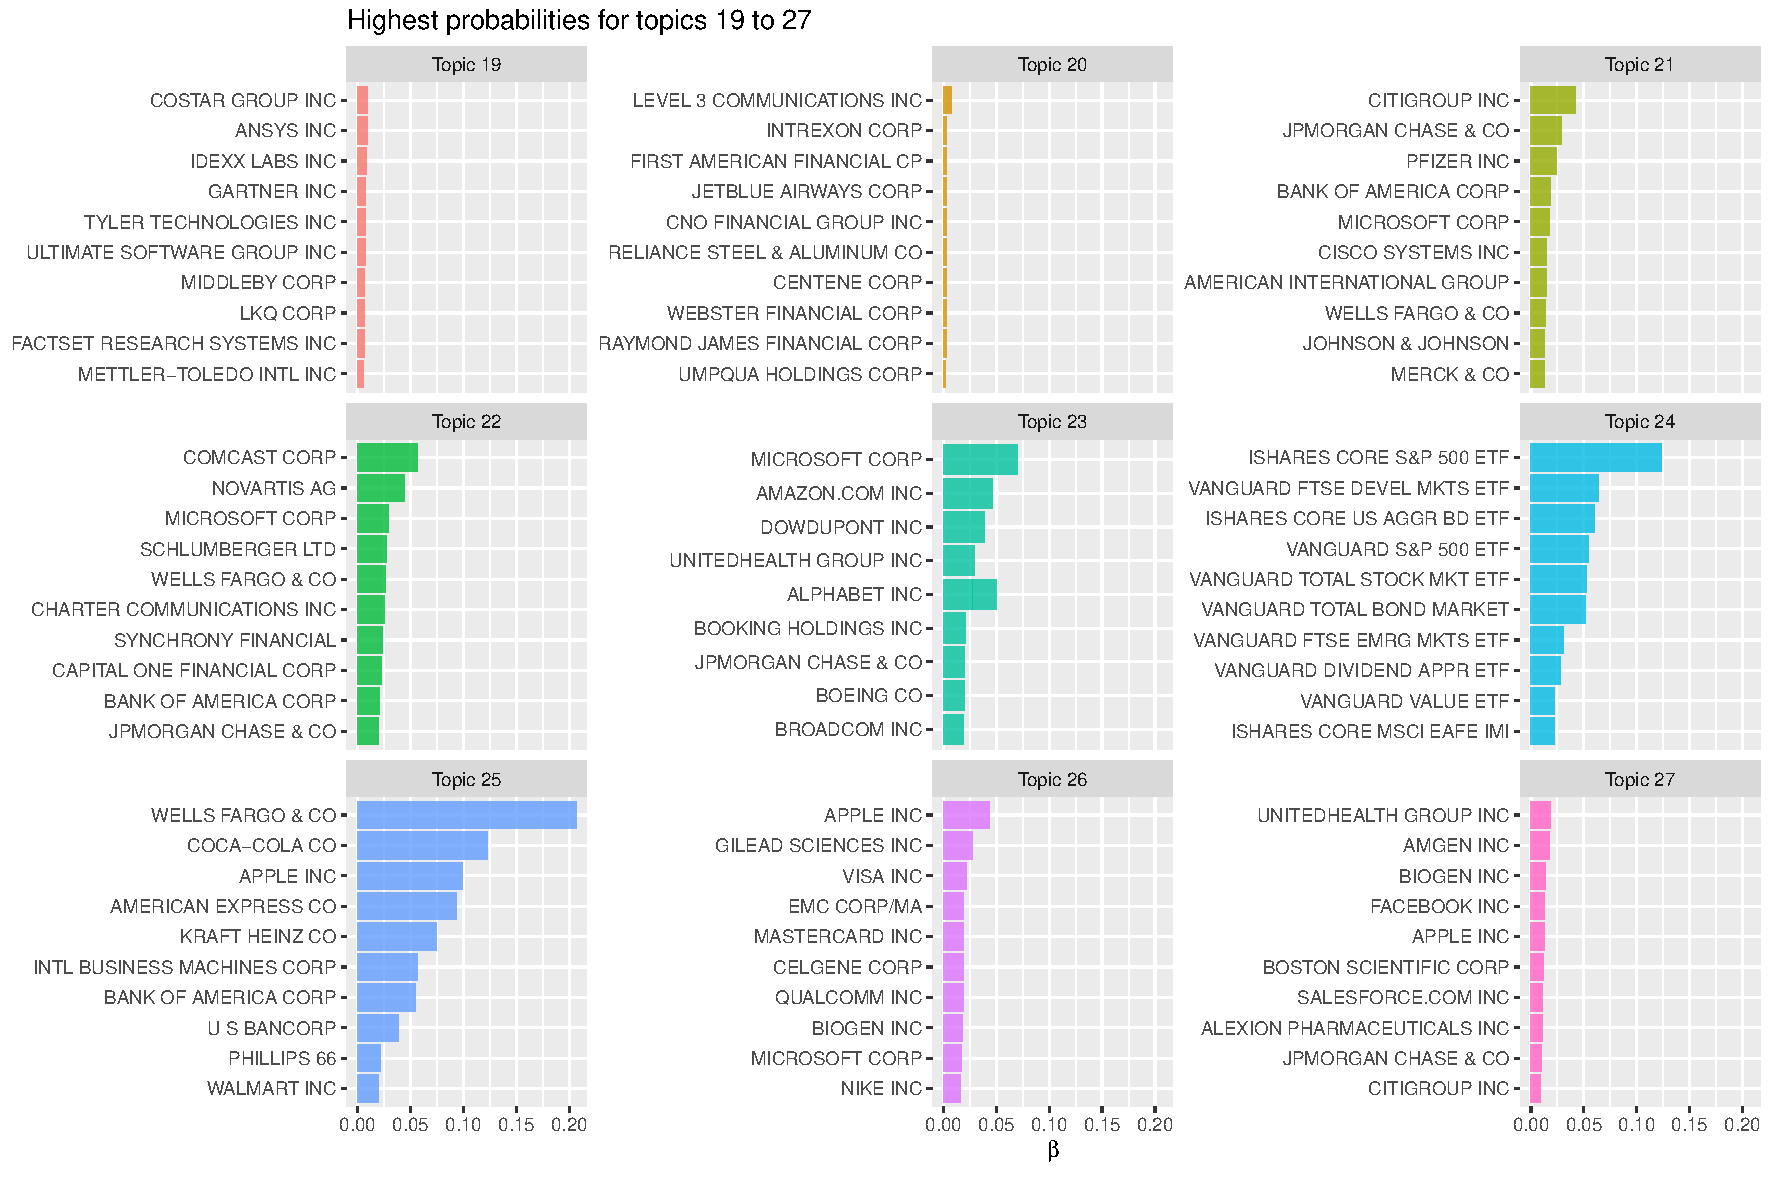
\includegraphics[width=1\linewidth]{Figures/ChapterV/LDA34_19_27}
	\caption[Topic Model with 34 Topics, Topics 19 thought 27]{Topic Model with 34 Topics,Topics 19 thought 27. This represents the 10 most likely stocks being associated to a particular portfolio archetype.}
	\label{fig:lda341927}
\end{figure}
	
\begin{figure}
	\centering
	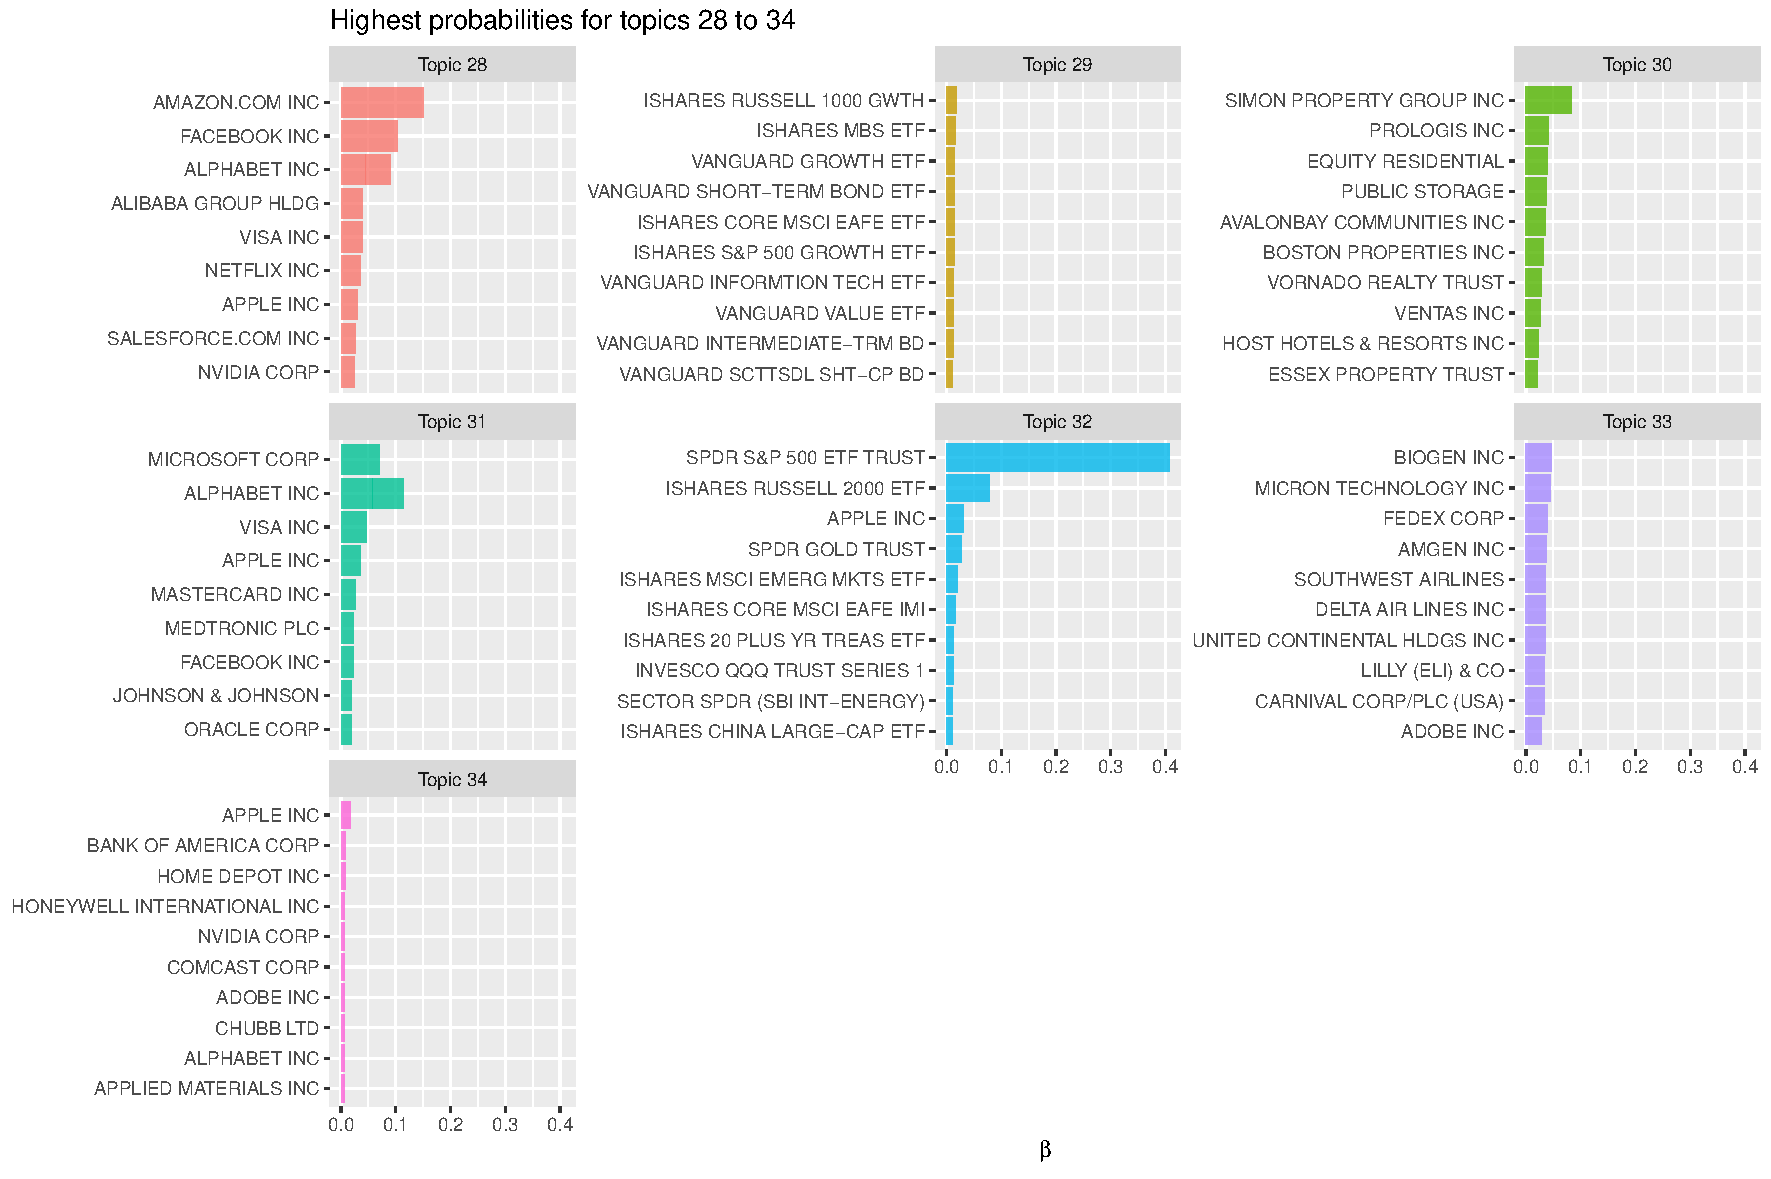
\includegraphics[width=1\linewidth]{Figures/ChapterV/LDA34_28_34}
	\caption[Topic Model with 34 Topics, Topics 28 thought 34]{Topic Model with 34 Topics, Topics 28 thought 34. This represents the 10 most likely stocks being associated to a particular portfolio archetype.}
	\label{fig:lda342834}
\end{figure}
	
\section{Shift-Share}

Shift share is a technique used in econometrics and regional studies to ascribe changes in the share of a particular sector of the local economy into 3 main factors: A national factor, that is to say how the global economy is doing, a industry factor, that is to say how well a particular industry is doing, and a regional factor, that is to say taking into account the national and industry trends, how well is an industry doing in a particular region.  This last factor is important, since it allows various regions to see how they are doing relative to the set of global and industry headwinds, such that for an industry in decline, a regional decline of 3\% in an industry declining 10\% with a national economy growing by 2\% is doing relatively well all things considered.  Similarly, the use of regional shifts to measure how well a region is doing with regards to an investment topic is useful for determining how well a given strategy is doing keeping the investment topic and the national trends. 

The equation for shift share is as follows:
\begin{equation}
   e^{t+n}_{i} - e^{t}_{i} = NS_{i} + IM_{i} + RS_{i}
    \label{Eq:Shft_share}
\end{equation}

Where $e$ is the shift share in industry $i$ between the time periods $t$ and $t+n$.  This shift share is the sum of the three effects: national growth effect ($NS_{i}$), the industry mix effect ($IM_{i}$) and the local shift ($RS_{i}$). 

The national share is calculated as follows:

\begin{equation}
    NS = e^{r}_{i}g^{n}
    \label{Eq:NationalShare}
\end{equation}

The industry mix is calculated as follows:
\begin{equation}
    IM = e^{r}_{i}(g^{n}_{i} - g^{n})
    \label{Eq:IndustryMix}
\end{equation}
and the regional shift is calculated as follows: 
\begin{equation}
    RS =  e^{r}_{i}(g^{r}_{i} - g^{n}_{i})
    \label{Eq:RegionalShare}
\end{equation}

Where $e^{r}_{i}$ is the value in Sector $i$ in Region $r$ at the beining of the period, $g^{n}$ is the growth rate for the value for the total area under study over the time period, $g^{n}_{i}$ is the growth rate of Sector $i$ for the total area under study for the time period, and $g^{r}_{i}$ growth rate in sector $i$ in Region $r$ for the time period. \citep{Houston67}. 

\subsection{Dynamic Shift Share}

However, as the release of data became more granular, both in terms of time period and geography, a more nuanced version of shift share was developed, the dynamic shift share.  This version of shift-share takes into account the period to period fluctuations by performing the shift-share in a time-series and adding together all of the shifts \citep{BarffKnight88}.  Since this model uses a time-series, it is less vulnerable to effects caused by choosing the start and end years. Furthermore, \cite{BarffKnight88} and \cite{harris1994dynamic} show that the use of a dyamic shift share with regular reporting periods (as is the case of 13F-HR data) means that there is less of a compounding effect.   

\begin{equation}
    e^{t+n}_{i} - e^{t}_{i} = NS_{i} + IM_{i} + RS_{i}
\end{equation}

If the study period rages from year $t$ to year $t+n$, the traditional shift-share effects are calculated for every year $k$, where k spans from $t+1$ to $t+n$. 

\begin{equation}
    NS_{i} = \sum_{k=t+1}^{t+n}[e^{k-1}_{i}(G^{k})]
    \label{Eq:NationalShare_dynamic}
\end{equation}

\begin{equation}
    IM_{i} = \sum_{k=t+1}^{t+n}[e^{k-1}_i(G^{k}_{i}-G^{k})]
     \label{Eq:IndustryMix_dynamic}
\end{equation}

\begin{equation}
    RS_{i} = \sum_{k=t+1}^{t+n}[e^{k-1}_i(g^{k}_{i} - G^{k}_{i} )]
        \label{Eq:RegionalShare_dynamic}
\end{equation}

For the dynamic model shift share, Equation \ref{Eq:NationalShare_dynamic} replaces Equation \ref{Eq:NationalShare} for the national share, Equation \ref{Eq:IndustryMix_dynamic} replaces Equation \ref{Eq:IndustryMix}  for the industry mix and Equation \ref{Eq:RegionalShare_dynamic} replaces Equation \ref{Eq:RegionalShare} for the regional share.  The dynamic model shift share is then calculated at the sum of the annual effects \citep{BarffKnight88}.  

In this case, rather than calculate yearly effects for $k$, this application of the dynamic shift share used each quarterly filing between the second quarter of 2013 to the fourth quarter of 2018, therefore creating 23 discreet time steps.

\todo{new material}
In order to get the values for the shift share, each 
\todo{end}
The analysis was performed using \cite{Soudis2019} R package implementation. The holdings of each portfolio was weighted by the $\beta$ of each topic/portfolio archetype as determined by the 34 topicLDA analysis, and summed by relevant geography.  For the initial use of the shift share, this is the State level. The results in tabular form can be found in Appendix \ref{appendix:shiftshare}.

By isolating the regional shifts and then mapping them onto a map of the USA we can isolate the local/regional effects of a given topic/portfolio archetype in a given geography while keeping the overall growth of the stock market and the varying popularity of a particular strategy constant. 

\subsection{A Word on Maps}

It should be noted that the maps in this chapter are not projected to accurately preserve distances or surface area, but are used more as cartogram showing the relative distribution of the regional shift by state.  Furthermore, while it is traditional to forgo the use of blue in a map to represent terrestrial areas since blue usually represents water and green usually represents landmasses, the \textit{viridis} colour pallet has been chosen since this colour pallet is usable by people with colourblindness, transfers readily to black and white printing, and more importantly offers a steady scaling between colour and the underlying value unlike a traditional red to violet colour pallet \citep{viridis2018}.    

\begin{figure}
	\centering
	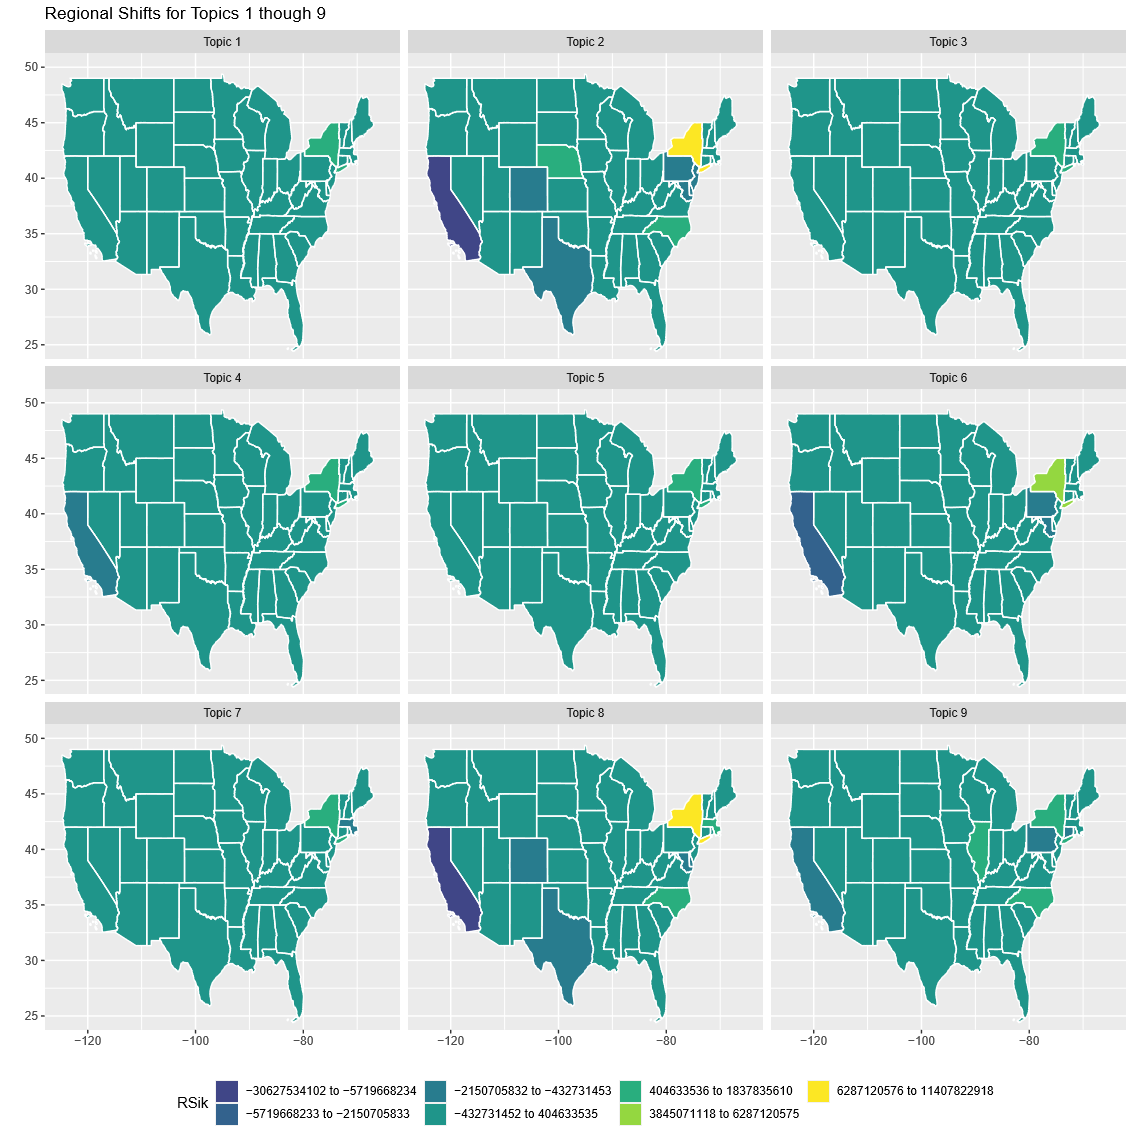
\includegraphics[width=1\linewidth]{Figures/ChapterV/States_01_09}
	\caption[Regional Shifts for Topics 1 to 9]{Regional Shifts for Topics 1 to 9.  Map is not to scale, but chosen to emphasise the relative distribution of regional shifts using the viridis colour scale.}
	\label{fig:states0109}
\end{figure}

\begin{figure}
	\centering
	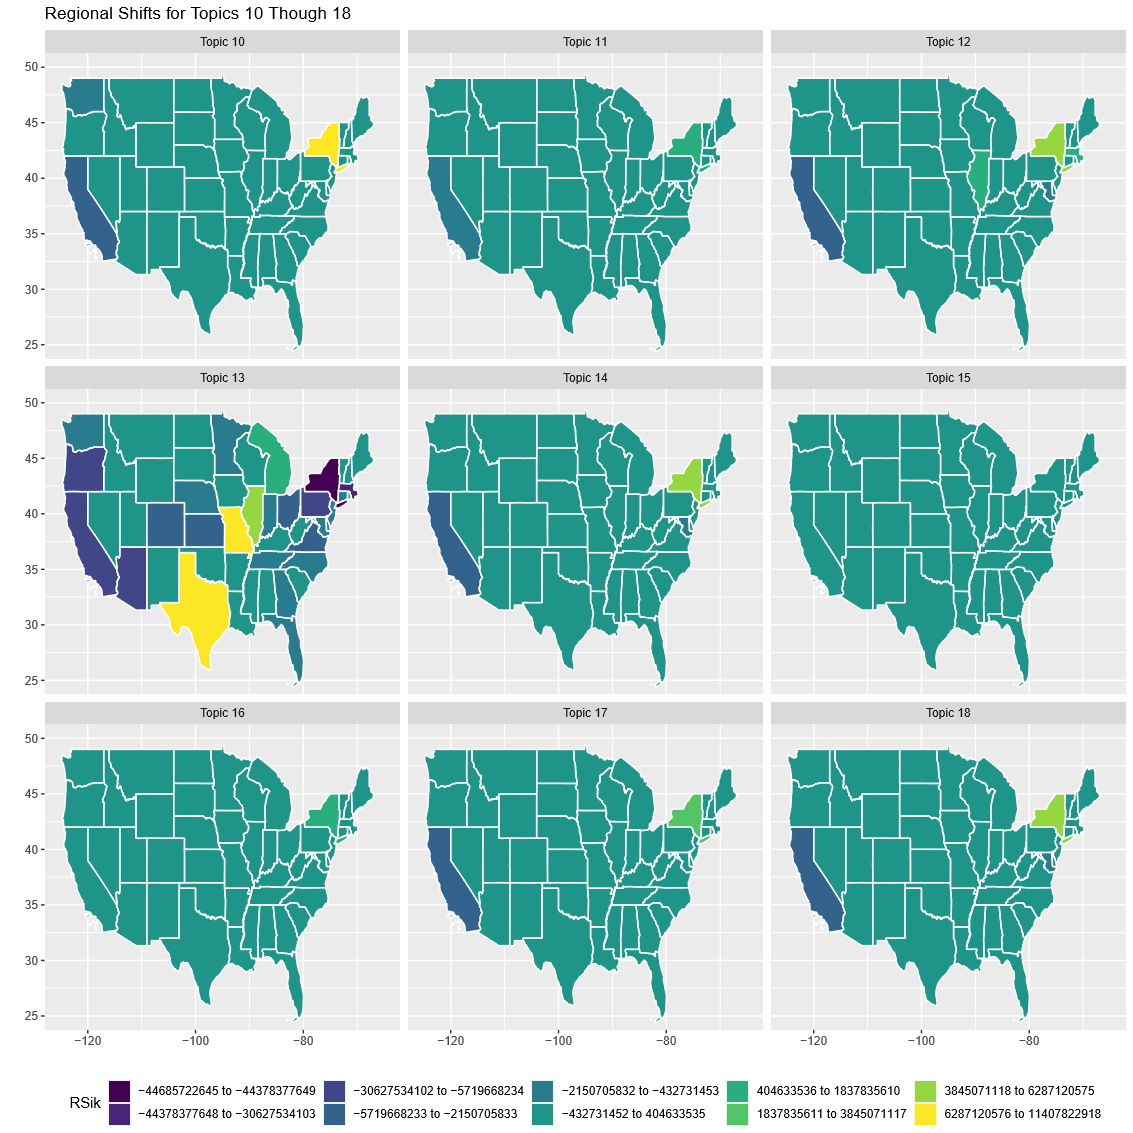
\includegraphics[width=1\linewidth]{Figures/ChapterV/States_10_18}
	\caption[Regional Shifts for Topics 9 to 18]{Regional Shifts for Topics 9 to 18}
	\label{fig:states10-18}
\end{figure}

\begin{figure}
	\centering
	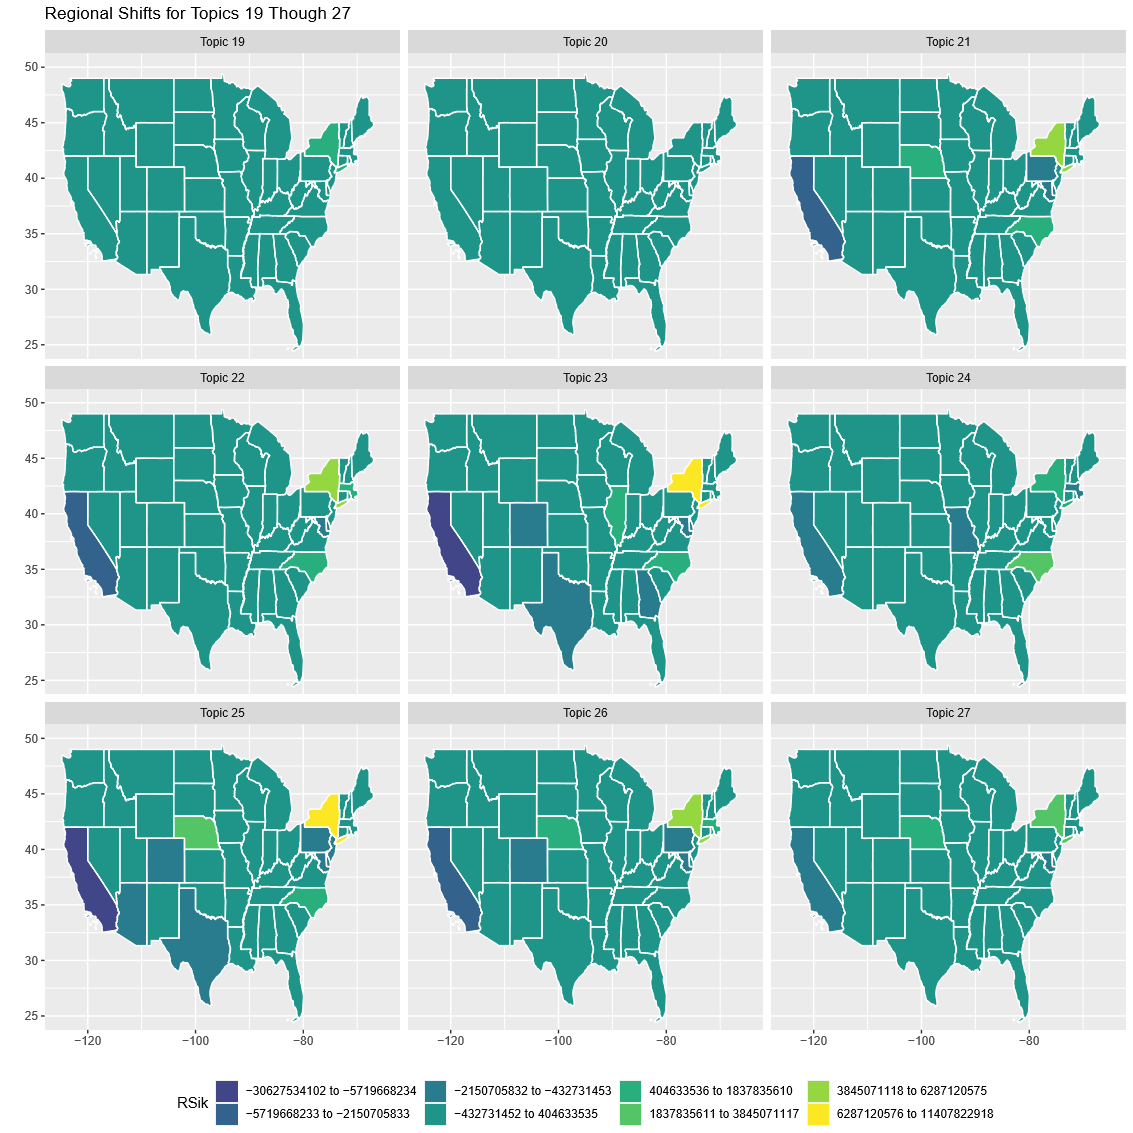
\includegraphics[width=1\linewidth]{Figures/ChapterV/States_19_27}
	\caption[Regional Shifts for Topics 19 to 27]{Regional Shifts for Topics 19 to 27}
	\label{fig:states19-27}
\end{figure}

\begin{figure}
	\centering
	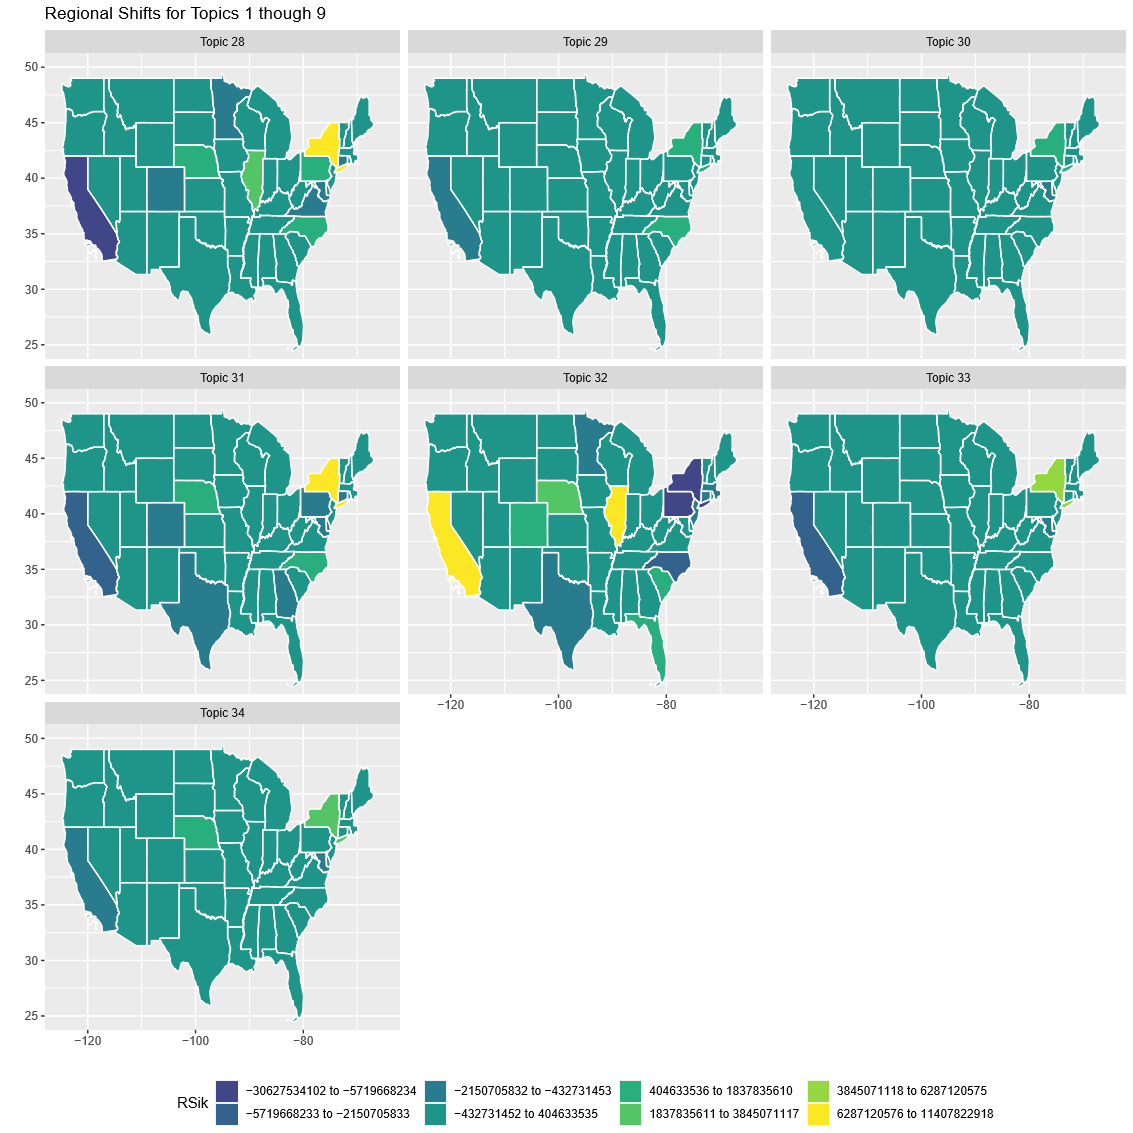
\includegraphics[width=1\linewidth]{Figures/ChapterV/States_28_34}
	\caption[Regional Shifts for Topics 19 to 27]{Regional Shifts for Topics 28 to 34}
	\label{fig:states28-34}
\end{figure}
	

Figures \ref{fig:states0109}, \ref{fig:states10-18}, \ref{fig:states19-27} and \ref{fig:states28-34} show a common pattern in which New York State and California are often on two sides of a continuum, with New York getting most of the growth of the dynamic regional shifts from 2013-2018, and California consistently under-performing.  That being said, New York isn't the only State that sees outsized growth in certain sectors, Illinois and California show growth above par in Topic 3,  Missouri with regards to Topic 25\footnote{to the point that it skews the colour balance of the other maps in Figure \ref{fig:states19-27} since they share a scale in a manner similar to how a bright object in a photograph washes out the details in the darker elements} (Berkshire Hathaway) and Topic 29 (Emerging Markets ETFs) in North Carolina.  Since the main players are New York State on the positive side and California on the negative side, insights on Topics 19 to 27 can be gleaned in section \ref{BattleoftheCoasts} and Appendix \ref{appendix:shiftshare}. 

-Topic 1 for a worked example:  

For topic 1 in California, the growth in the National holdings of 13F holders accounts for a growth of 5358.96 (what does this mean???)  

New York 

National shift:  5089.85
Industry shift: -3004.34
Regional shift:  5847.87

California:  
National Shift:  5358.96
Industry Shift: -2302.8
Regional Shift: -3389.5

This shows New York to be way more dynamic and central in the investment world, across nearly all strategies. This lead to the paradoxical outcome in which institutional investment is following a 40+ year old trend of diffusion due to lower barriers of entry, seeing that the greatest monetary gains across each strategy shows that the directors of institutional investments still consider New York to be their nexus.  






\section{Battle of the Coasts}
\label{BattleoftheCoasts}
As seen in the previous section, the largest contrast in strategies lies in New York State and California.  Diving into the data in a more granular way shows that most of this contrast is driven by the differences between the CBSAs of New York and San Francisco, as well as occasionally Los Angeles.  In some sense, this isn't really surprising considering the relevant literature \todo{citations} on the subject of different investment culture between the East Coast and the West Coast.  In fact, this in some ways, can been seen as a continuation of the different coastal cultures between the more buttoned up east coast, centred around the Boston Highway 128 Research Cluster, and the more freewheeling, and casual dress of Silicone Valley.  And not to put too much emphasis on this, but the West Coast does have an affinity for tech stocks that isn't shared by New York City.  

While it would be possible to do a straight comparison of New York State with California, there are a few factors that suggest against this.  First of all, this would ignore the contributions to the New York CBSA from the New Jersey side of the Hudson River, in particular the contributions of Hudson County New Jersey, home to many back-office financial functions as well as a fair number of smaller investors (between 3 to 11 depending on the time period (Appendix \ref{Appendix:Countycount})) in suburban office  parks \citep{gongthe2012}.  On the other hand, a map of California can be useful for both the San Francisco and Los Angeles CBSAs since all of the affected counties (San Francisco, San Mateo and LA Counties) are located in the State of California.  


Unsurprisingly, New York County (Manhattan) is the key driver of the concentration for New York State and the New York CBSA.  As mentioned previously in Chapter \ref{ChapterIIIb} and with quarter to quarter counts in Appendix \ref{App:CountiesCount}, New York County is at the head of the US institutional investor count urban hierarchy, and this is a position that while somewhat eroding, will continue to be unquestioned for the foreseeable future.  

While it would be expected that if local knowledge wasn't a factor amongst many when deciding where to invest, there wouldn't be any locally-sourced tacit knowledge to guide investments, all regions and New York County in particular would be a blend of most strategies.  Therefore, this coastal difference suggest that tacit knowledge plays a part in investing. As such, this is suggestive that \cite{Graves2003} is correct in raising the question about the applicability of geographically-based knowledge and the Efficient Market Hypothesis.  More to the point, the EMH, especially in the strong and medium form, might not be applicable in reality due to information asymmetries driven by locally sourced tacit knowledge.  Whether or not investors use this tacit knowledge primarily in the growth position, the hedge, or across their portfolio can be left to future work.  

The only county in the New York CBSA that has a large regional shift other than New York County is Westchester County with regards to Topic 31 (E-commerce and Bio-med), which has a large under-shift, meaning that this county is less invested in a strategy than would be expected given the other factors in the shift share.  This is in contrast to the previously mentioned Hudson County, yet it does not have a significant shift.  Two explanations for the lack of large regional shits for this area include the low dollar value in aggregate, since the county consists of small investors, and the highly diversified strategy - therefore giving relatively small regional shifts since they don't deviate much from what would be expected of them.  

The examples of Westchester and Hudson counties, as well as the non-factors of King County (Brooklyn) which contain many small investors re-enforce the notion that while there might be an increase in count of suburban institutional investors, they don't really shift the centre of gravity from the large concentrations in the large CBDs. 

California: 

Mostly driven by SF. Except for Topic 3 in SF, California has no positive shifts.   





LA county plays an occasional role.  Comparable to Boston or Chicago.  

The first major point of contrast between New York and SF is Topic 3 (Market tracking ETFs).  These are great ways capture the growth of a stock market, in this case the S\&P 500, in a passive way and little to no need to tacit knowledge.  Similarly, the large under shift in Topic 4 (Banks and Blue Chips) have a New York feel, and no surprise, NYC has a high share, while SF has a low share.  


	
\begin{figure}
	\centering
	\includegraphics[width=1\linewidth]{Figures/ChapterV/NY_01_09}
	\caption[Regional Shifts for Topics 1 to 9]{Regional Shifts for Topics 1 to 9}
	\label{fig:NYC0109}
\end{figure}

\begin{figure}
	\centering
	\includegraphics[width=1\linewidth]{Figures/ChapterV/Cali_01_09}
	\caption[Regional Shifts for Topics 1 to 9]{Regional Shifts for Topics 1 to 9}
	\label{fig:SF0109}
\end{figure}
	


\begin{figure}
	\centering
	\includegraphics[width=1\linewidth]{Figures/ChapterV/NY_10_18}
	\caption[Regional Shifts for Topics 9 to 18]{Regional Shifts for Topics 9 to 18}
	\label{fig:NYC10-18}
\end{figure}

\begin{figure}
	\centering
	\includegraphics[width=1\linewidth]{Figures/ChapterV/Cali_10_18}
	\caption[Regional Shifts for Topics 9 to 18]{Regional Shifts for Topics 9 to 18}
	\label{fig:CA10-18}
\end{figure}

\begin{figure}
	\centering
	\includegraphics[width=1\linewidth]{Figures/ChapterV/NY_19_27}
	\caption[Regional Shifts for Topics 19 to 27]{Regional Shifts for Topics 19 to 27}
	\label{fig:NYC19-27}
\end{figure}

\begin{figure}
	\centering
	\includegraphics[width=1\linewidth]{Figures/ChapterV/Cali_19_27}
	\caption[Regional Shifts for Topics 19 to 27]{Regional Shifts for Topics 19 to 27}
	\label{fig:CA19-27}
\end{figure}


\begin{figure}
	\centering
	\includegraphics[width=1\linewidth]{Figures/ChapterV/NY_28_34}
	\caption[Regional Shifts for Topics 19 to 27]{Regional Shifts for Topics 28 to 34}
	\label{fig:NYC28-34}
\end{figure}


\begin{figure}
	\centering
	\includegraphics[width=1\linewidth]{Figures/ChapterV/Cali_28_34}
	\caption[Regional Shifts for Topics 19 to 27]{Regional Shifts for Topics 28 to 34}
	\label{fig:CA28-34}
\end{figure}


